\documentclass[tikz,border=3pt,convert={density=600,outext=.png}]{standalone}
%\documentclass[tikz,border=3pt]{standalone}

\usepackage[T2A]{fontenc}       			%поддержка кириллицы
\usepackage[utf8]{inputenc} % utf8 encoding
\usepackage{amsmath,amsfonts} % nice math symbols

\usepackage{tikz}
\usetikzlibrary{arrows,shapes,calc,patterns}

\begin{document}
	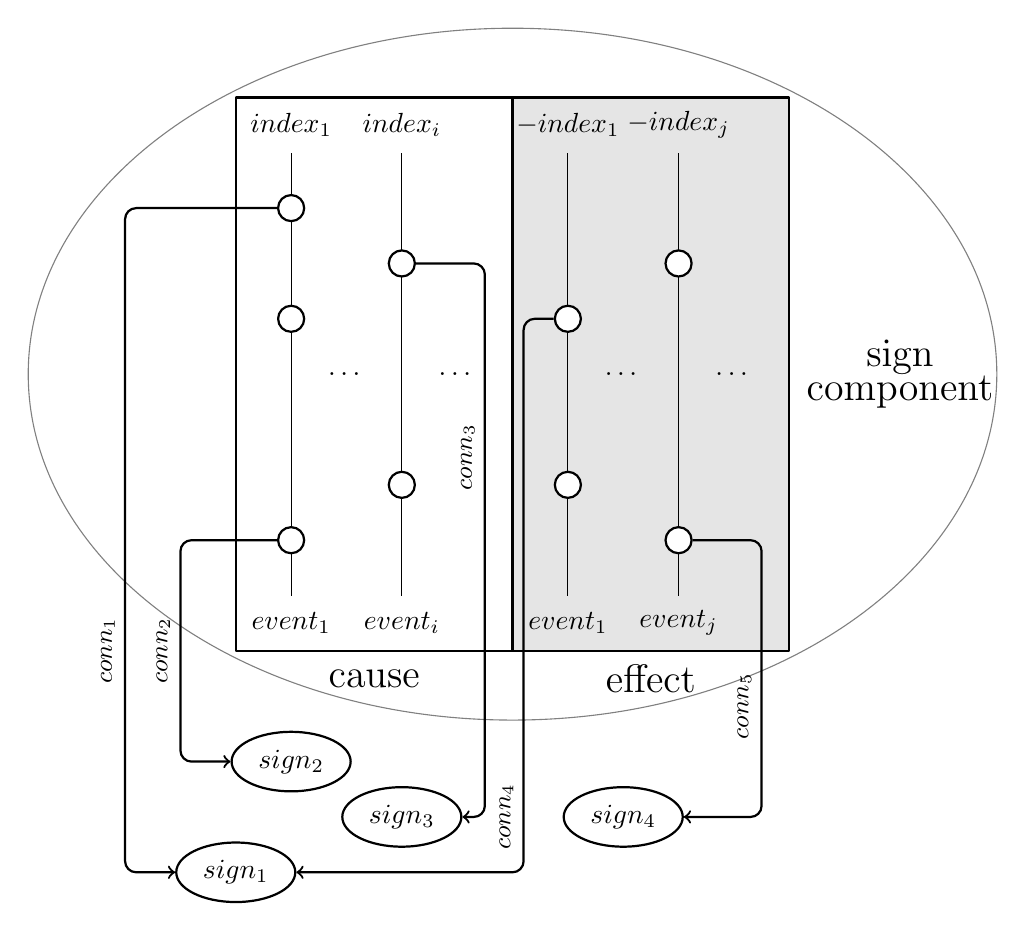
\begin{tikzpicture}[join=round,scale=2.0]
		\tikzstyle{ell}=[draw, thick, align=center]
		
		\node[draw, thin,gray, ellipse, minimum width = 350pt, minimum height = 250pt] at (50pt, 50pt)  {};
		\node[align=center] at (120pt, 50pt) {\Large sign\\\Large component};
		\draw[ell] (0,0) rectangle (50 pt, 100 pt);
		\draw[ell, fill=white!90!black] (50 pt,0) rectangle (100 pt, 100 pt);
		\draw[ell, very thick] (50 pt, 0) -- (50 pt, 100 pt);
		\draw (10 pt, 10 pt) -- (10 pt, 90 pt);
		\node at (20 pt, 50 pt) {$\dots$};
		\draw (30 pt, 10 pt) -- (30 pt, 90 pt);
		\node at (40 pt, 50 pt) {$\dots$};
		
		\draw (60 pt, 10 pt) -- (60 pt, 90 pt);
		\node at (70 pt, 50 pt) {$\dots$};
		\draw (80 pt, 10 pt) -- (80 pt, 90 pt);
		\node at (90 pt, 50 pt) {$\dots$};
		
		\node[ell, fill=white, circle, minimum size=2 pt] (p1) at (10 pt, 20 pt) {};
		\node[ell, fill=white, circle, minimum size=2 pt] (p2) at (10 pt, 60 pt) {};
		\node[ell, fill=white, circle, minimum size=2 pt] (p3) at (10 pt, 80 pt) {};
		\node[ell, fill=white, circle, minimum size=2 pt] (p4) at (30 pt, 30 pt) {};
		\node[ell, fill=white, circle, minimum size=2 pt] (p5) at (30 pt, 70 pt) {};
		
		\node[ell, fill=white, circle, minimum size=2 pt] (p6) at (60 pt, 30 pt) {};
		\node[ell, fill=white, circle, minimum size=2 pt] (p7) at (60 pt, 60 pt) {};
		\node[ell, fill=white, circle, minimum size=2 pt] (p8) at (80 pt, 20 pt) {};
		\node[ell, fill=white, circle, minimum size=2 pt] (p9) at (80 pt, 70 pt) {};
		
		\node at (10 pt, 95 pt) {$index_1$};
		\node at (30 pt, 95 pt) {$index_i$};
		\node at (60 pt, 95 pt) {$-index_1$};
		\node at (80 pt, 95 pt) {$-index_j$};
		
		\node at (10 pt, 5 pt) {$event_1$};
		\node at (30 pt, 5 pt) {$event_i$};
		\node at (60 pt, 5 pt) {$event_1$};
		\node at (80 pt, 5 pt) {$event_j$};
		
		\node at (25 pt, -5 pt) {\Large cause};
		\node at (75 pt, -5 pt) {\Large effect};
				
		\node[ell, ellipse] (s1) at (0, -40pt)  {$sign_1$};
		\node[ell, ellipse] (s2) at (10pt, -20pt)  {$sign_2$};
		\node[ell, ellipse] (s3) at (30pt, -30pt)  {$sign_3$};
		\node[ell, ellipse] (s4) at (70pt, -30pt)  {$sign_4$};
		\draw[ell, ->,rounded corners] (p3.west) -| (-20pt, 0) node[above, rotate=90] {\small $conn_1$} |- (s1);
		\draw[ell, ->,rounded corners] (p1.west) -| (-10pt, 0) node[above, rotate=90] {\small $conn_2$} |- (s2);
		\draw[ell, ->,rounded corners] (p5.east) -| (45pt, 0) node[above, rotate=90, near end] {\small $conn_3$} |- (s3);
		
		\draw[ell, ->,rounded corners] (p7.west) -| (52pt, 0) |- node[yshift=20pt, above, rotate=90] {\small $conn_4$} (s1);
		\draw[ell, ->,rounded corners] (p8.east) -| (95pt, 0) node[yshift=-20pt,above, rotate=90] {\small $conn_5$} |- (s4);
	\end{tikzpicture}
\end{document}